
\section{ICO learning parameters}
\label{app:appendixICO}

\subsection{ICO learning}
The input correlation learning rule by \citet{Porr2006ICO} is a Heterosynaptic
learning rule, it is unsupervised and performs a correlation between a predefined reflex signal
($x_{0}$) and a reflex predicting signal ($x_{1}$). Hence, this learning
algorithm identifies and exploits causalities between temporal
sequential signals.

\begin{figure}[htbp]
\begin{center}
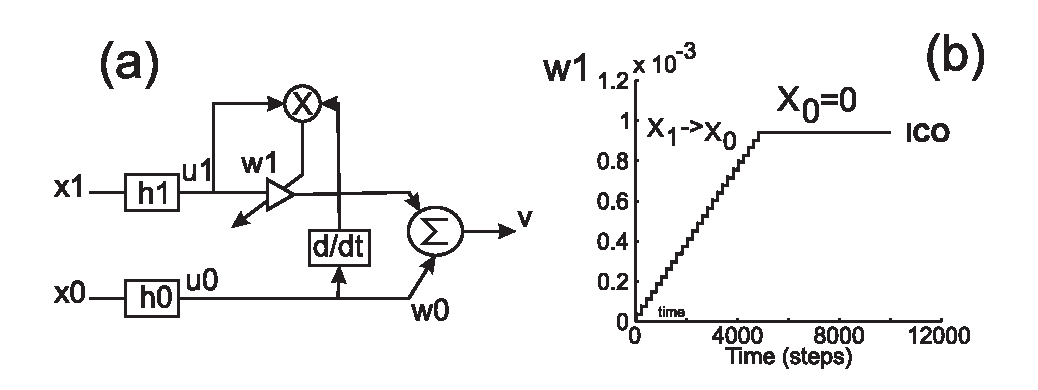
\includegraphics[scale=0.5]{figures/socialadapt/ico.eps}
\caption[Agent learns with the ICO learning]{Figure (a) shows the ICO learning basic
block composed by 2 inputs $x_{0},x_{1}$ filtered by $h_{0},h_{1}$ and the output $v$.
Figure (b) shows the weight change of $w_{1}$ during time. At the beginning $w_{1}=0$,
then for 5000 simulation steps $x_{1}$ anticipates $x_{0}$ and the $w_{1}$ grows until 1.0.
After 5000 simulation steps reflex is suppressed $x_{0}=0$ and $w_{1}$ stabilize to $1 \cdot 10^{-3}$.
\label{fig:appendix.ICO}}
\end{center}
\end{figure}

Figure \ref{fig:appendix.ICO} shows the ico learning block which has two inputs $x_{0}$,$x_{1}$
from the agent's sensor that are filtered by bandpass filters $h_{0},h_{1}$.
The transfer function $h$ is a bandpass which transforms
a d-pulse input into a damped oscillation and is specified in the
Laplace-domain:
\begin{equation}
h(t) \leftrightarrow H(s) =\frac{1}{(s+p)(s+p*)}
\end{equation}
where $p*$ represents the complex conjugate of the pole $p = a + ib$. It is
important to note that such a bandpass is only stable if its pole-pair is
located on the left complex half-plane, otherwise an amplified oscillation is
obtained.

\begin{eqnarray}
h(t)&=&\frac{1}{b}e^{at}sin(bt)\\
a&=&-\pi \frac{F}{Q}\\
b&=&\sqrt{(2\pi F)^2 -a^{2}}
\end{eqnarray}

$F$ is the oscillation frequency and $Q$ the quality factor.
The damping characteristic of the filter is reflected by $Q$ (see Appendix A).
Filtered signals $u_{i}(t)$ are transferred with weight $w_{i}$ to the output
neurons. In the output neuron the output $v(t)$ is calculated by
summing up all incoming signals according to their weights:
\begin{equation}
v(t)=\sum_{k=0}^{1}w_{k}u_{k}
\end{equation}
which represent the input for the motor system.
The unsupervised character of the ICO learning rule is reached by
the synaptic weight $w_{1}$ to be adapted by the weight
change rule:
\begin{equation}
\frac{d}{dt}w_{1}=\mu u_{1} \frac{d u_{0}}{dt}
\end{equation}
The weight change is dependent on the derivative of the reflex input
signal $u_{0}$, the input signal $u_{1}$ and a
learning rate $\mu$. The
learning rule has been shown to be useful for avoidance and attraction
mechanisms and has fast and stable convergence \citep{Porr2006ICO}.

The filter response $h$ is parametric in $Q$.
If $Q>\infty$ it means that:
\begin{itemize}
\item $a=0$
\item $b=2 \pi f$
\end{itemize}
therefore the filter response becomes
$H(s)=\frac{1}{(s^2-(2* \pi *f)^2)}$
that is a resonator with frequency $2 \pi f$, see Fig. \ref{fig:qinf}.
When $Q$ approaches 0, $Q \rightarrow 0$ this is the result:
$H(s)=\frac{1}{(s^2+2as+2a^2)}$
a trinomial term with infinite cutoff frequency, see Fig. \ref{fig:qzero}.

\begin{figure*}
\centerline{
\subfigure[Bode diagram of $h$ filter when $Q>\infty$]{
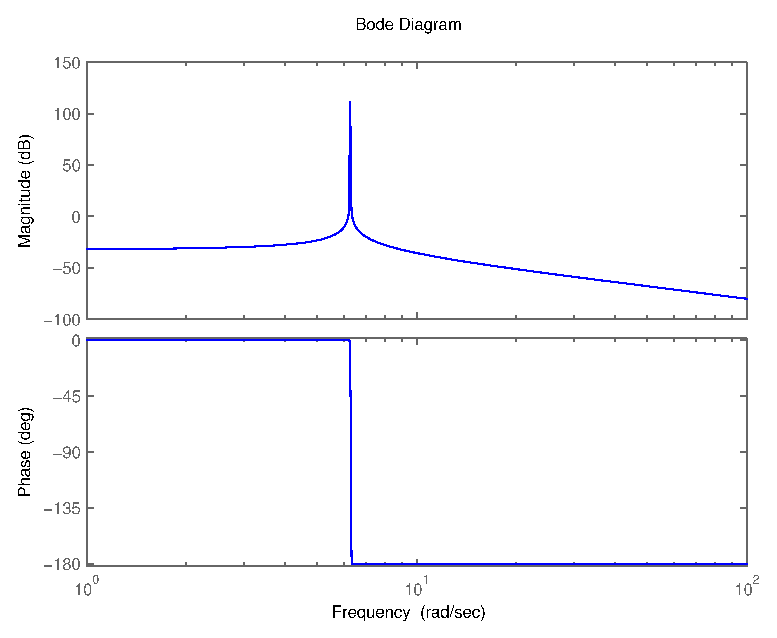
\includegraphics[scale=0.4]{figures/infomeasure/Qinf.eps}
\label{fig:qinf}}
\hfil
\subfigure[Bode diagram of $h$ filter when $Q \rightarrow 0$]{
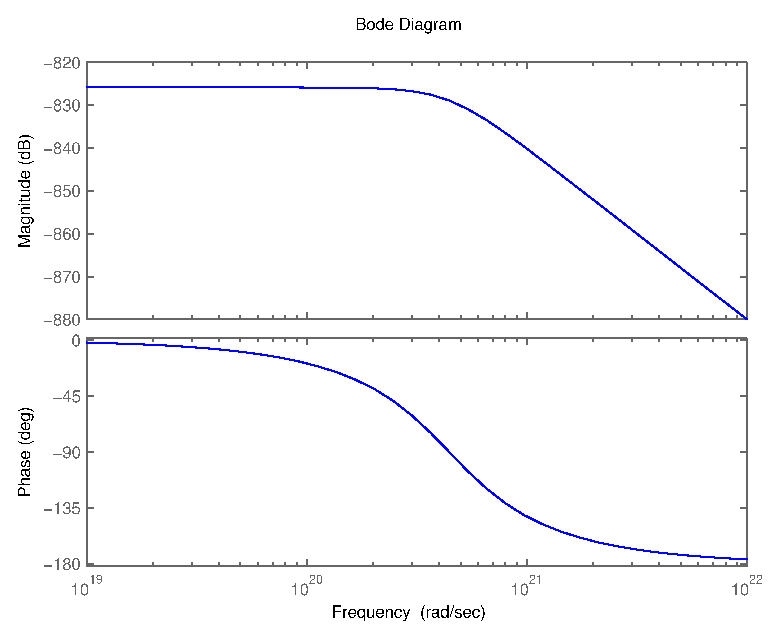
\includegraphics[scale=0.4]{figures/infomeasure/Qzero.eps}
\label{fig:qzero}}}
\caption[Bode diagrams for different Q values]{Bode diagrams for different Q values. \label{fig:ICOfilter}}
\end{figure*}

When $Q=1/\sqrt(2)$ the filter has a maximally flat response without any overshoot.
When $Q \leq 0.5$ the filter has no undershoot in the impulse response.
